%!TEX root = ../ltransform.tex
% \section{Введение}
\addcontentsline{toc}{section}{Введение}
\section*{Введение}
% \vspace{-0.5em}
В данной работе исследуется преобразование структуры лазерного излучения. Рассматриваются два метода: метод \textit{попутного двухволнового взаимодействия} и \textit{обращение волнового фронта (ОВФ) при четырехволновом смешении}, основанные на интерференции монохроматических волн в нелинейной среде $\varepsilon(|\vec{E}|)$. В такой среде не выполняется принцип суперпозиции, а распространение волны в такой среде можно рассматривать как самодифракцию на периодической структуре $\varepsilon$, которая порождается распространяющимися в нелинейной среде волнами. 

Целью работы является знакомство с нелинейной интерференцией волн. Предполагается изучить проявление эффекта обращения волнового фронта при четырехволновом смешении волн в нелинейных жидких кристаллах.
% В настоящей работе изучаются два наиболее эффективных и известных метода преобразования структуры лазерного излучения оптического диапазона: метод попутного двухволнового взаимодействия (ПДВ) и метод обращения волнового фронта при четырехволновом смешении (ОВФ при ЧВС). Оба метода основаны на явлении интерференции волн монохроматического излучения в нелинейной среде, свойства которой и, прежде всего, диэлектрическая проницаемость $\varepsilon$ зависят от величины амплитуды действующего поля $|\vec{E}|$. По существу в нелинейной среде волны, имеющие достаточно большую интенсивность поля, начинают взаимодействовать между собой. В результате такого взаимодействия, осуществляемого через посредство нелинейной среды, изменяются характеристики волн и, как следствие, свойства самой среды. В свою очередь, изменяющиеся свойства нелинейной среды влияют на условия распространения излучения и возможности дальнейшей трансформации его структуры. Фактически в нелинейной среде происходит взаимодействие излучения с веществом. Самым очевидным следствием взаимодействия излучения с веществом является нарушение принципа суперпозиции в его простейшем представлении, когда две волны теряют способность распространяться независимо друг от друга.

% Любая пара волн образует в нелинейной среде периодически изменяющуюся в пространстве составляющую $\varepsilon$, на которой каждая из волн рассеивается (дифрагирует) по нескольким направлениями и, в частности, по двум основным направлениям распространения. Рассеяние каждой волны на периодической структуре $\varepsilon$ аналогично по своей сути дифракции волны, распространяющейся в свободном пространстве, на фиксированной антенной решётке, находящейся на пути её распространения. Поэтому явление рассеивания (или перерассеивания) волн на <<решётке>> диэлектрической проницаемости $\varepsilon$ можно назвать самодифракцией оптического излучения в нелинейной среде или нелинейной интерференцией (нелинейным сложением) волн. В этой связи важной частью настоящей работы является близкое знакомство с нелинейной интерференцией двух волн, которое должно стать ключевым моментом в изучении теории взаимодействия излучения с веществом.



\section{Метод попутного двухволнового взаимодействия}
В среде со слабой нелинейностью структуры взаимодействующих волн могут меняться слабо, но при этом в определённых условиях может происходить перераспределение их интенсивностей. С таким явлением связана возможность передачи энергии мощного лазерного пучка, форма волнового фронта которого подлежит коррекции, опорному пучку с малой начальной интенсивностью и плоским волновым фронтом. В этом заключена практическая значимость явления попутного двухволнового взаимодействия (далее -- ПДВ). В настоящем разделе теоретически будет показана возможность реализации ПДВ в жидкой (или газообразной) движущейся проводящей среде с так называемым тепловым механизмом нелинейности, который обусловлен разогревом среды.

\begin{figure}[ht]
	\centering
	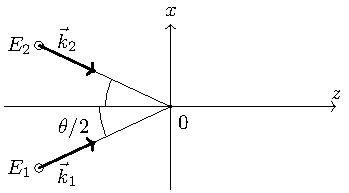
\includegraphics[scale=1.5]{fig/fig1.pdf}
	\caption{Две волны в среде}
	\label{fig:figure1}
\end{figure}

Рассмотрим распространение двух плоских монохроматических волн
\begin{equation}
	\label{eq:pdv.1}
	\vec{E}_{1,2}=\operatorname{Re}\left\{\vec{y}_{0} \tilde{E}_{1,2}(z) \cdot \exp \left[i\left(-k_{z} z \mp k_{x} x+\omega t\right)\right]\right\}
\end{equation}
в однородном изотропном полупространстве $z>0$ (Рис. \ref{fig:figure1}) движущейся с постоянной скоростью $v_0 \vec{x}_0$ жидкой (или газообразной) среды, имеющей линейную диэлектрическую проницаемость $\varepsilon_0$ и проводимость $\sigma_0$. Падающие из вакуума на границу среды волны поляризованы перпендикулярно плоскости падения. Внутри среды их волновые векторы $\vec{k}_{1,2} = \pm k_x \vec{x}_0 + k_z \vec{z_0}$, направленные симметрично относительно оси OZ, имеют составляющие
\begin{equation}
	\label{eq:pdv.2}
	k_{x}=k_{0} \sin (\theta / 2) \equiv(\omega / c) \sin (\theta / 2) ; \quad k_{z}=\sqrt{k_{0}^{2} \varepsilon_{0} \mu-k_{x}^{2}} \equiv \sqrt{k^{2}-k_{x}^{2}}.
\end{equation}
Трансформация комплексной амплитуды поля в среде описывается скалярным волновым уравнением Гельмгольца
\begin{equation}
	\label{eq:pdv.3}
	\Delta \tilde{E}+k^{2} \tilde{E}-\frac{i \omega}{c^{2}} \mu 4 \pi \sigma_{0} \tilde{E}=-\omega^{2} \mu \frac{4 \pi}{c^{2}} \tilde{P}^\text{nl},
\end{equation}
где $\sigma_{0}$ - проводимость среды, $\mu$ - магнитная проницаемость, $\tilde{P}^\text{nl}$ - комплексная амплитуда нелинейной поляризации среды (предполагается, что $\vec{P}^\text{nl} \upuparrows \vec{E}$).

За счет пространственно неоднородного тепловыделения в интерференционном поле $\overline{|\vec{E}|}^{({2\pi}/{\omega})}$ двух разнонаправленных волн в проводящей среде возникает тепловая решетка с периодом $\Lambda = \pi / k_x$, равным периоду интерференционной картины. Тепловая решетка формирует нелинейную поляризацию среды
\begin{equation}
	\label{eq:pdv.4}
	\tilde{P}^\text{nl}=\frac{\delta \varepsilon}{4 \pi} \tilde{E}
\end{equation}
и тем самым создаёт нелинейную часть $\delta \varepsilon$ её диэлектрической проницаемости $\varepsilon = \varepsilon_0 + \delta\varepsilon$.


\subsection{Модель теплового механизма нелинейности}
Как известно, все процессы и все движения в жидкости (или газе) описываются уравнениями гидродинамики. Они отражают законы сохранения массы, импульса и энергии элементарной жидкой частицы и в наиболее общем случае могут быть представлены в виде системы трёх уравнений
\begin{equation}
	\label{eq:pdv.5}
	\frac{\partial \rho}{\partial t}+\operatorname{div}(\rho \vec{v})=0,
\end{equation}
\begin{equation}
	\label{eq:pdv.6}
	\frac{\partial \vec{v}}{\partial t}+(\vec{v} \cdot \nabla) \vec{v}=-\frac{\nabla p}{\rho}+\vec{g}-\frac{\nabla V}{\rho}+\frac{\operatorname{div} \hat{\sigma}}{\rho},
\end{equation}
\begin{equation}
	\label{eq:pdv.7}
	\rho T\left[\frac{\partial S}{\partial t}+(\vec{v} \cdot \nabla S)\right]=(\hat{\sigma} \cdot \nabla) \vec{v}+\operatorname{div}(\kappa \nabla T)+\overline{\Pi}^{(2 \pi / \omega)},
\end{equation}
в которых $\rho$ - плотность среды, $p$ - давление, $\vec{v}$ - скорость движения элементарного объёма жидкости, $T$ - температура, $S$ - энтропия, $\vec{g}$ - ускорение свободного падения, $\kappa$ - коэффициент теплопроводности среды,
\begin{equation}
	\label{eq:pdv.8}
	\overline{\Pi}^{(2 \pi / \omega)}=\sigma_{0} \overline{|\vec{E}|^{2}}^{(2 \pi / \omega)}-\left[\frac{T}{8 \pi}\left(\frac{\partial \varepsilon}{\partial T}\right)_{p}\right]_{0} \frac{\partial}{\partial T} \overline{|\vec{E}|^{2}}^{(2 \pi / \omega)}
\end{equation}
-- мощность индуцированных полем источников тепла (второе слагаемое учитывает электрокалорический эффект), $\hat{\sigma}$ - тензор вязких напряжений, связанный со скоростью дифференциальным соотношением
\begin{equation}
	\label{eq:pdv.9}
	\operatorname{div} \hat{\sigma}=\eta \Delta \vec{v}+[(\eta / 3)+\zeta](\nabla \cdot \operatorname{div} \vec{v}),
\end{equation}
где $\eta$, $\zeta$ - коэффициенты вязкости,
\begin{equation}
	\label{eq:pdv.10}
	V=-\frac{1}{8 \pi}\left(\rho \frac{\partial \varepsilon}{\partial \rho}\right)_{S} \overline{|\vec{E}|^{2}}^{(2 \pi / \omega)}
\end{equation}
-- потенциальная энергия электрострикции. Система материальных уравнений \eqref{eq:pdv.5} -- \eqref{eq:pdv.7} включает в себя также уравнение состояния среды, которое может связывать любые три величины из полного набора переменных термодинамических величин и зависит от условий эксперимента. В частности, уравнение состояния среды может иметь одну из возможных форм
\begin{equation}
	\label{eq:pdv.11}
	\rho=f_{1}(p, T) ; \quad S=f_{2}(p, T).
\end{equation}
Система материальных уравнений \eqref{eq:pdv.5} - \eqref{eq:pdv.7} и \eqref{eq:pdv.11} совместно с уравнением Гельмгольца \eqref{eq:pdv.3} для электромагнитного поля является замкнутой и полной для описания взаимодействия монохроматического лазерного излучения с жидкой нелинейной средой. В разных (по химическому составу) средах и в различных экспериментальных условиях отдельные компоненты материальных уравнений могут вносить пренебрежимо малые вклады в описание нелинейных явлений. В частности, при описании стационарного ПДВ можно не учитывать вклада в нагревание среды электрокалорического эффекта \eqref{eq:pdv.8}. Учитывая, что характерное время формирования нелинейной поляризации намного больше времени, за которое звуковая волна успевает пробежать период возникающей в среде тепловой решетки и выровнять давление в среде, можно и нужно пренебречь энергией электрострикции \eqref{eq:pdv.10}, т.е. третьим членом в правой части уравнения \eqref{eq:pdv.6}.

В практически реализуемых условиях жидкость (или газ) оказывается средой со слабой нелинейностью, и воздействие лазерного излучения на такую среду проявляется в виде весьма малых отклонений термодинамических величин $\rho$, $p$, $S$, $T$, $\vec{v}$ от их стационарных невозмущенных значений. Поэтому почти все регистрируемые нелинейные эффекты, включая ПДВ, с большой точностью можно описывать материальными уравнениями для возмущений термодинамических величин среды.


Считая возмущения $\tilde{\rho}$, $\tilde{p}$, $\tilde{S}$, $\tilde{T}$, $\vec{\tilde{v}}$, вносимые полем в среду, малыми по сравнению с невозмущёнными стационарными значениями $\rho_0$, $p_0$, $S_0$, $T_0$, $\vec{v}_0$, вначале линеаризуем уравнения \eqref{eq:pdv.5}, \eqref{eq:pdv.6} и преобразуем их в уравнения
\begin{equation}
	\label{eq:pdv.12}
	\frac{\partial \tilde{\rho}}{\partial t}+\operatorname{div}\left(\rho_{0} \vec{\tilde{v}}\right)+\operatorname{div}\left(\tilde{\rho} \vec{v}_{0}\right)=0,
\end{equation}
\begin{equation}
	\label{eq:pdv.13}
	\rho_{0}\left(\frac{\partial \vec{\tilde{v}}}{\partial t}\right)+\rho_{0}\left(\vec{v}_{0} \cdot \nabla\right) \vec{v}=-\nabla \tilde{p}+\frac{1}{\rho_{0}}\left\{\eta \Delta \rho_{0} \vec{v}+[(\eta / 3)+\zeta] \nabla \operatorname{div}\left(\rho_{0} \vec{v}\right)\right\}.	
\end{equation}
Применим операцию дивергенции к уравнению \eqref{eq:pdv.13} и, используя \eqref{eq:pdv.12} в виде
\begin{equation}
	\label{eq:pdv.12'}
	\operatorname{div}\left(\rho_{0} \vec{\tilde{v}}\right)=-\frac{\partial \tilde{\rho}}{\partial t}-\left(\vec{v}_{0} \cdot \nabla \tilde{\rho}\right),
\end{equation}
получим уравнение
\begin{equation}
	\label{eq:pdv.14}
	\left[\frac{\partial}{\partial t}+\left(\vec{v}_{0} \cdot \nabla\right)-\frac{1}{\rho_{0}}\left(\frac{4 \eta}{3}+\zeta\right) \Delta\right]\left\{\frac{\partial \tilde{\rho}}{\partial t}+\left(\vec{v}_{0} \cdot \nabla \tilde{\rho}\right)\right\}=\Delta \tilde{p},
\end{equation}
которое связывает изменения плотности среды $\tilde{\rho}$ и давления в ней $\tilde{p}$.

Поскольку экспериментально измеряются изменения давления и температуры, то уравнение \eqref{eq:pdv.14} следует трансформировать так, чтобы оно описывало связь возмущений термодинамических величин $p$ и $T$. Это нетрудно сделать, используя одно из возможных уравнений состояния среды, связывающее плотность, давление и температуру. Линеаризуя первое уравнение \eqref{eq:pdv.11} вблизи состояния равновесия, получим связь между изменениями плотности, давления и температуры
\begin{equation}
	\label{eq:pdv.15}
	\tilde{\rho}=\left(\frac{\partial f_{1}}{\partial p}\right)_{p_{0}, T_{0}} \tilde{p}+\left(\frac{\partial f_{1}}{\partial T}\right)_{p_{0}, T_{0}} \tilde{T},
\end{equation}
которая позволяет (путём исключения $\tilde{\rho}$) преобразовать \eqref{eq:pdv.14} в уравнение
\begin{equation}
	\label{eq:pdv.16}
	\begin{array}{l}
	\left(\frac{\partial f_{1}}{\partial p}\right)_{p_{0}, T_{0}}\left[\frac{\partial}{\partial t}+\left(\vec{v}_{0} \cdot \nabla\right)-\frac{1}{\rho_{0}}\left(\frac{4 \eta}{3}+\zeta\right) \Delta\right]\left\{\frac{\partial \tilde{p}}{\partial t}+\left(\vec{v}_{0} \cdot \nabla \tilde{p}\right)\right\}-\Delta \tilde{p}+ \\
	+\left(\frac{\partial f_{1}}{\partial T}\right)_{p_{0}, T_{0}}\left\{\frac{\partial}{\partial t}+\left(\vec{v}_{0} \cdot \nabla\right)-\frac{1}{\rho_{0}}\left(\frac{4 \eta}{3}+\zeta\right) \Delta\right\}\left[\frac{\partial \tilde{T}}{\partial t}+\left(\vec{v}_{0} \cdot \nabla \tilde{T}\right)\right]=0
\end{array}
\end{equation}
относительно возмущений давления и температуры. Эксперимент проводится в условиях постоянного давления ($p = \mathrm{const} = p_0 $), когда все переходные процессы завершены и потому отсутствуют вариации давления ($\tilde{p}=0$). Поэтому \eqref{eq:pdv.16} приобретает вид уравнения
\begin{equation}
	\label{eq:pdv.17}
	\left\{\frac{\partial^{2}}{\partial t^{2}}+\frac{\partial}{\partial t}\left(\vec{v}_{0} \cdot \nabla\right)+\left(\vec{v}_{0} \cdot \nabla\right)^{2}-\frac{1}{\rho_{0}}\left(\frac{4 \eta}{3}+\zeta\right) \Delta\left[\frac{\partial}{\partial t}+\left(\vec{v}_{0} \cdot \nabla\right)\right]\right\} \tilde{T}=0,
\end{equation}
в котором отсутствуют источники для роста температуры. Это означает, что материальные уравнения \eqref{eq:pdv.5} и \eqref{eq:pdv.6} не вносят никакого вклада в тепловую нелинейность проводящей среды.

Обратимся к материальному уравнению \eqref{eq:pdv.7}, которое является следствием закона сохранения энергии элементарного объёма среды. Линеаризуя \eqref{eq:pdv.7} вблизи стационарных значений термодинамических величин, получим уравнение
\begin{equation}
	\label{eq:pdv.18}
	\rho_{0} T_{0}\left[\frac{\partial \tilde{S}}{\partial t}+\left(\vec{v}_{0} \cdot \nabla \tilde{S}\right)\right]=(\hat{\sigma} \cdot \nabla) \vec{\tilde{v}}+\operatorname{div}(\kappa \nabla \tilde{T})+\sigma_{0} \overline{|\vec{E}|^{2}}^{(2\pi/\omega)},
\end{equation}
описывающее изменения энтропии и температуры. Поскольку тепловыделение, обусловленное внутренним трением, пропорционально членам второго порядка малости по возмущению скорости $\vec{\tilde{v}}$ и практически ничтожно мало по сравнению с тепловыделением при поглощении, то число членов в правой части \eqref{eq:pdv.18} можно и нужно уменьшить до двух, избавившись от $(\hat{\sigma} \cdot \nabla)\vec{\tilde{v}}$.

Уравнение \eqref{eq:pdv.18} следует преобразовать в уравнение, связывающее возмущения давления и температуры. Для этого необходимо использовать другую линеаризованную форму уравнения \eqref{eq:pdv.11} состояния среды
\begin{equation}
	\label{eq:pdv.19}
	\tilde{S}=\left(\frac{\partial f_{2}}{\partial p}\right)_{p_{0}, T_{0}} \tilde{p}+\left(\frac{\partial f_{2}}{\partial T}\right)_{p_{0}, T_{0}} \tilde{T}.
\end{equation}
Подставляя \eqref{eq:pdv.19} в \eqref{eq:pdv.18}, получим уравнение для возмущений давления и температуры
\begin{equation}
	\label{eq:pdv.20}
	\rho_{0} C_{p}\left[\frac{\partial \tilde{T}}{\partial t}+\left(\vec{v}_{0} \cdot \nabla \tilde{T}\right)\right]+\rho_{0} T_{0}\left[\frac{\partial \tilde{p}}{\partial t}+\left(\vec{v}_{0} \cdot \nabla \tilde{p}\right)\right] \cdot\left(\frac{\partial \tilde{S}}{\partial \tilde{p}}\right)_{T}=\kappa \Delta \tilde{T}+\sigma_{0} \overline{|\vec{E}|^{2}}^{(2 \pi / \omega)},
\end{equation}
в котором использовано понятие теплоёмкости при постоянном давлении $C_p = T_0 (\partial S  / \partial T)_p  = T_0 (\partial f_2  / \partial T)_p$. При условии $p = \mathrm{const} = p_0 $ ($\tilde{p}=0$) уравнение \eqref{eq:pdv.20} трансформируется в уравнение для температуры
\begin{equation}
	\label{eq:pdv.21}
	\left[\frac{\partial \tilde{T}}{\partial t}+\left(\vec{v}_{0} \cdot \nabla \tilde{T}\right)\right]-\chi \Delta \tilde{T}=\frac{\sigma_{0}}{\rho_{0} C_{p}} \overline{|\vec{E}|^{2}}^{(2 \pi / \omega)},
\end{equation}
которое описывает изменение $\tilde{T}$ в среде, имеющей коэффициент температуропроводности
\begin{equation}
	\label{eq:pdv.22}
	\chi=\left(\kappa / \rho_{0} C_{p}\right).
\end{equation}
Источником температуры в правой части \eqref{eq:pdv.21} являются тепловые потери в проводящей среде. Температуропроводность среды -- это следствие потока тепла из-за наличия градиента температуры.



\subsection{Стационарное взаимодействие двух попутных волн}

В общем случае для корректного решения уравнения \eqref{eq:pdv.21} необходимо задать граничные и начальное условия. В случае ПДВ из-за отсутствия конкретных сведений о форме и температуре поверхности трубы, в которой течёт жидкость, граничные условия для уравнения теплопроводности можно учесть приближенно. Для этого достаточно ввести в его левую часть дополнительный член $\tilde{T} / \tau_0$, формально учитывающий теплообмен с окружающей средой. 
Феноменологически вводимую в уравнение \eqref{eq:pdv.21} величину $\tau_0^{-1}$ называют коэффициентом потери температуры в результате теплоотвода.

Начальное условие необходимо для описания процесса изменения
температуры текущей жидкости $\tilde{T}(t)$ во времени, например, с целью изучения механизмов формирования ПДВ. В этом случае начальным условием было бы естественно считать $\tilde{T}(t=0) = 0$. Для описания стационарного ПДВ, когда процесс изменения температуры прекратился и можно положить $(\partial \tilde{T}  / \partial t) = 0$, начальное условие оказывается излишним.

Малая нелинейная часть диэлектрической проницаемости $\delta \varepsilon$, которая образуется в проводящей среде из-за изменения температуры и давления, в общем случае может быть представлена в виде
\begin{equation}
	\label{eq:pdv.23}
	\delta \varepsilon=\left(\frac{\partial \varepsilon}{\partial T}\right)_{p} \tilde{T}+\left(\frac{\partial \varepsilon}{\partial p}\right)_{T} \tilde{p}.
\end{equation}
В установившемся (стационарном) режиме ПДВ, когда $p=\mathrm{const}$ и $\tilde{p} = 0$, образовавшаяся в проводящей среде нелинейная часть диэлектрической проницаемости $\delta \varepsilon$ с точностью до постоянного коэффициента совпадает с возмущением температуры $\tilde{T}$:
\begin{equation}
	\label{eq:pdv.24}
	\delta \varepsilon=(\partial \varepsilon / \partial T)_{p} \tilde{T}.
\end{equation}
Таким образом, в стационарном случае с учётом потери температуры из-за теплоотвода и с помощью \eqref{eq:pdv.24} уравнение \eqref{eq:pdv.21} преобразуется в уравнение
\begin{equation}
	\label{eq:pdv.25}
	\frac{\delta \varepsilon}{\tau_{0}}+\left(\overrightarrow{v}_{0} \cdot \nabla \delta \varepsilon\right)-\frac{\kappa}{\rho_{0} C_{p}} \Delta \delta \varepsilon=\frac{\sigma_{0}}{\rho_{0} C_{p}} \cdot\left(\frac{\partial \varepsilon}{\partial T}\right)_{p} \overline{|\vec{E}|^{2}}^{(2 \pi / \omega)}
\end{equation}
относительно нелинейной диэлектрической проницаемости $\delta \varepsilon$. Её пространственная структура формируется средней за период $(2 \pi / \omega)$ интенсивностью
\begin{equation}
	\label{eq:pdv.26}
	\overline{|\vec{E}|^{2}}^{(2 \pi / \omega)}=\frac{1}{2} \cdot\left\{\left|\tilde{E}_{1}(z)\right|^{2}+\left|\tilde{E}_{2}(z)\right|^{2}+\left[\tilde{E}_{1}(z) \tilde{E}_{2}^{*}(z) \exp \left(-i 2 k_{x} x\right)+\text{ к. с.}\right]\right\}
\end{equation}
интерференционного поля $\vec{E}$ двух волн с медленно меняющимися вдоль координаты $z$ комплексными амплитудами $\tilde{E}_{1,2}(z)$. Изменение комплексной амплитуды поля $\tilde{E}$ описывается скалярным уравнением Гельмгольца \eqref{eq:pdv.3}, которое с учётом \eqref{eq:pdv.2} и \eqref{eq:pdv.4} приобретает форму
\begin{equation}
	\label{eq:pdv.27}
	\Delta \tilde{E}+k^{2} \tilde{E}-i k^{2} \frac{4 \pi \sigma_{0}}{\varepsilon_{0} \omega} \tilde{E}=-k^{2} \frac{\delta \varepsilon}{\varepsilon_{0}} \tilde{E}.
\end{equation}
Уравнения \eqref{eq:pdv.25} и \eqref{eq:pdv.27} образуют замкнутую систему. Анализ этой пары уравнений позволяет вполне однозначно определить пространственную структуру нелинейной диэлектрической проницаемости в виде
\begin{equation}
	\label{eq:pdv.28}
	\delta \varepsilon=\delta \varepsilon^{\prime \prime}(z)+\left[\delta \tilde{\varepsilon}(z) \cdot \frac{1}{2} \cdot \exp \left(-2 i k_{x} x\right)+\text{ к. с.}\right],
\end{equation}
где средняя составляющая $\delta \varepsilon'' (z)$  и комплексная амплитуда $\delta \tilde{\varepsilon}$ решётки $\delta \varepsilon$ по координате $x$ являются медленно меняющимися на длине волны $\lambda = 2\pi / k$ функциями координаты $z$.

Подставляя \eqref{eq:pdv.28} в \eqref{eq:pdv.25} и используя ортогональность пространственных гармоник $\delta \varepsilon$ по координате $x$, нетрудно получить уравнения для средней составляющей   $\delta \varepsilon'' (z)$ и комплексной амплитуды $\delta \tilde{\varepsilon}$ решётки нелинейной диэлектрической проницаемости
\begin{equation}
	\label{eq:pdv.29}
	\frac{1}{\tau_{0}} \delta \varepsilon^{\prime \prime}(z) \cong \frac{\sigma_{0}}{2 \rho_{0} C_{p}}\left(\frac{\partial \varepsilon}{\partial T}\right)_{p}\left(\left|\tilde{E}_{1}\right|^{2}+\left|\tilde{E}_{2}\right|^{2}\right),
\end{equation}
\begin{equation}
	\label{eq:pdv.30}
	\left[-i {v}_{0} 2 k_{x}+\frac{\kappa 4 k_{x}^{2}}{\rho_{0} C_{p}}+\frac{1}{\tau_{0}}\right] \delta 
	\tilde{\varepsilon}(z) \cong \frac{\sigma_{0}}{\rho_{0} C_{p}} \cdot\left(\frac{\partial \varepsilon}{\partial T}\right)_{p} \tilde{E}_{1} \tilde{E}_{2}^{*}.
\end{equation}
При выводе \eqref{eq:pdv.29} и \eqref{eq:pdv.30} опущены малые члены ($d^2 \delta \varepsilon'' (z) / d z^2$) и ($d^2 \delta \tilde\varepsilon (z) / d z^2$)‚ что и определяет приближённый характер этих уравнений.

Подставляя поле $\tilde{E}$ в виде суммы волн \eqref{eq:pdv.1} в уравнение Гельмгольца \eqref{eq:pdv.27}
и используя ортогональность их полей по координате $x$ ‚ можно получить систему из двух связанных уравнений для комплексных амплитуд $\tilde{E}_{1,2}(z)$
\begin{equation}
	\label{eq:pdv.31}
	-2 i k_{z} \frac{\partial \tilde{E}_{1}}{\partial z}-i k^{2} \frac{4 \pi \sigma_{0}}{\varepsilon_{0} \omega} \tilde{E}_{1} \cong-\frac{k^{2}}{\varepsilon_{0}}\left\{\delta \varepsilon^{\prime \prime} \cdot \tilde{E}_{1}+\frac{1}{2} \delta \tilde{\varepsilon} \cdot \tilde{E}_{2}\right\},
\end{equation}
\begin{equation}
	\label{eq:pdv.32}
	-2 i k_{z} \frac{\partial \tilde{E}_{2}}{\partial z}-i k^{2} \frac{4 \pi \sigma_{0}}{\varepsilon_{0} \omega} \tilde{E}_{2} \cong-\frac{k^{2}}{\varepsilon_{0}}\left\{\delta \varepsilon^{\prime \prime} \cdot \tilde{E}_{2}+\frac{1}{2} \delta \tilde{\varepsilon}^{*} \cdot \tilde{E}_{1}\right\},
\end{equation}
из которых исключены как ничтожно малые члены ($d^2 \tilde{E}_{1,2} / dz^2$).

Уравнения \eqref{eq:pdv.29} -- \eqref{eq:pdv.32} образуют систему с большим числом коэффициентов разной размерности, что препятствует выявлению физической природы и
оценкам величин основных параметров механизма ПДВ. С целью упрощения
записи уравнений целесообразно ввести безразмерные амплитуды волн поля
\begin{equation}
	\label{eq:pdv.33}
	\tilde{\mathcal{E}}_{1,2}=\left(\tilde{E}_{1,2} / \sqrt{\left|\tilde{E}_{1}(0)\right|^{2}}\right) \equiv\left(\tilde{E}_{1,2} / \sqrt{I_{0}}\right)
\end{equation}
и их интенсивности 
\begin{equation}
	\label{eq:pdv.34}
	\tilde{\mathcal{E}}_{1,2} \cdot \tilde{\mathcal{E}}_{1,2}^* \equiv \mathcal{E}_{1,2}^{2},
\end{equation}
безразмерную координату
\begin{equation}
	\label{eq:pdv.35}
	\xi = z \cdot \frac{k^2}{k_z \varepsilon_0},
\end{equation}
безразмерный коэффициент затухания поля в проводящей среде
\begin{equation}
	\label{eq:pdv.36}
	\gamma = \frac{4\pi \sigma_0}{\omega}
\end{equation}
и следующие физические параметры: обусловленное коэффициентами теплоотвода $1/\tau_0$ и температуропроводности ($\chi = [\kappa / \rho_0 C_p]$) среды время
\begin{equation}
	\label{eq:pdv.37}
	\tau_\text{r} = \frac{\tau_0}{1+4\chi k_x^2 \tau_0},
\end{equation}
имеющее смысл времени релаксации решётки диэлектрической проницаемости
при описании нестационарного ПДВ, безразмерный параметр
\begin{equation}
	\label{eq:pdv.38}
	\delta = v_0 2 k_x \tau_\text{r},
\end{equation}
определяющий величину пространственного смещения решётки диэлектрической проницаемости относительно интерференционной картины распределения
интенсивности поля в среде, безразмерный параметр нелинейности среды
\begin{equation}
	\label{eq:pdv.39}
	G = \frac{\sigma_0 \tau_\text{r} I_0}{4 \varepsilon_0 \rho_0 C_p} \left(\frac{\partial \varepsilon}{\partial T}\right)_p,
\end{equation}
характеризующий эффективность ПДВ. В безразмерном виде уравнения \eqref{eq:pdv.29} -- \eqref{eq:pdv.32} примут компактную форму
\begin{equation}
	\label{eq:pdv.40}
	\delta \varepsilon^{\prime \prime}=2 G\left(\tau_{0} / \tau_{\mathrm{r}}\right) \cdot\left({\mathcal { E }}_{1}^{2}+\mathcal{E}_{2}^{2}\right), 
\end{equation}
\begin{equation}
	\label{eq:pdv.41}
	\delta \tilde{\varepsilon}=\frac{4 G}{1+i \delta} \cdot \tilde{\mathcal{E}}_{1} \tilde{\mathcal{E}}_{2}^{*},
\end{equation}
\begin{equation}
	\label{eq:pdv.42}
	\left[\frac{d}{d \xi}+\frac{\gamma}{2}\right] \tilde{\mathcal{E}}_{1}=\frac{-i}{2} \cdot\left(\delta \varepsilon^{\prime \prime} \cdot \tilde{\mathcal{E}}_{1}+\frac{1}{2} \delta \tilde{\varepsilon} \cdot \tilde{\mathcal{E}}_{2}\right),
\end{equation}
\begin{equation}
	\label{eq:pdv.43}
	\left[\frac{d}{d \xi}+\frac{\gamma}{2}\right] \tilde{\mathcal{E}}_{2}=\frac{-i}{2} \cdot\left(\delta \varepsilon^{\prime \prime} \cdot \tilde{\mathcal{E}}_{2}+\frac{1}{2} \delta \tilde{\varepsilon}^{*} \cdot \tilde{\mathcal{E}}_{1}\right).
\end{equation}

Подставляя выражения $\delta \varepsilon'' (z)$ из \eqref{eq:pdv.40} и $\delta \tilde{\varepsilon}$ из \eqref{eq:pdv.41} в \eqref{eq:pdv.42} и \eqref{eq:pdv.43}, нетрудно получить два связанных симметричных уравнения 
\begin{equation}
	\label{eq:pdv.44}
	\left[\frac{d}{d \xi}+\frac{\gamma}{2}+i 2 G \frac{\tau_{0}}{\tau_{\mathrm{r}}} \cdot\left({\mathcal { E }}_{1}^{2}+{\mathcal { E }}_{2}^{2}\right)\right] \tilde{\mathcal{E}_{1}}=\frac{-i G}{1+i \delta} \cdot \mathcal{E}_{2}^{2} \tilde{\mathcal{E}}_{1},
\end{equation}
\begin{equation}
	\label{eq:pdv.45}
	\left[\frac{d}{d \xi}+\frac{\gamma}{2}+i 2 G \frac{\tau_{0}}{\tau_{\mathrm{r}}} \cdot\left({\mathcal { E }}_{1}^{2}+{\mathcal { E }}_{2}^{2}\right)\right] \tilde{\mathcal{E}}_{2}=\frac{-i G}{1-i \delta} \cdot \mathcal{E}_{1}^{2} \tilde{\mathcal{E}}_{2}
\end{equation}

относительно амплитуд $\tilde{\mathcal{E}}_{1,2}$ взаимодействующих между собой волн. Механизмом взаимодействия является дифракция (или рассеяние) волн на решётке диэлектрической проницаемости среды. Механизм взаимодействия волн и пределы его возможностей становятся более понятными, если от \eqref{eq:pdv.44} и \eqref{eq:pdv.45} перейти к уравнениям для интенсивностей ${\mathcal{E}}_{1,2}^2$.


Уравнения для интенсивностей взаимодействующих волн
\begin{equation}
	\label{eq:pdv.46}
	{\left[\frac{d}{d \xi}+\gamma \right] \mathcal{E}_{1}^{2}=\frac{-2 \delta G}{1+\delta^{2}} \cdot \mathcal{E}_{2}^{2} \mathcal{E}_{1}^{2}},
\end{equation}
\begin{equation}
	\label{eq:pdv.47}
	\left[\frac{d}{d \xi}+\gamma \right] \mathcal{E}_{2}^{2}=\frac{2 \delta G}{1+\delta^{2}} \cdot \mathcal{E}_{1}^{2} \mathcal{E}_{2}^{2}
\end{equation}
имеют одинаковые по величине и противоположные по знаку правые части. Это значит, что в случае
\begin{equation*}
	\delta G > 0
\end{equation*}
интенсивность волны ${\mathcal{E}}_{2}^2$ будет приобретать дополнительную энергию в результате рассеяния на решётке $\delta \varepsilon$ в направлении $\vec{k}_2$ взаимодействующей с ней и теряющей свою энергию первой волны. Если дополнительная энергия $2\delta G \cdot \mathcal{E}_1^2 \cdot \mathcal{E}_2^2 / (1+\delta^2)$, которую получает вторая волна от первой, будет больше энергии $\gamma \mathcal{E}_2^2$, которую она теряет из-за наличия линейного поглощения, то интенсивность $\mathcal{E}_2^2$ будет расти. Наибольшая эффективность перекачки энергии при прочих равных условиях будет иметь место при $|\delta| = 1$, и, следовательно, оптимальная скорость течения среды составляет
\begin{equation}
	\label{eq:pdv.48}
	(v_0)_\text{opt} = \frac{1}{2 k_x \tau_\text{r}}.
\end{equation}
При этом интенсивность $\mathcal{E}_1^2$ волны-донора согласно \eqref{eq:pdv.44} монотонно уменьшается. Т.e., условие роста интенсивности $\mathcal{E}_2^2$ волны-акцептора
\begin{equation}
	\label{eq:pdv.49}
	2 \delta G \cdot \mathcal{E}_{1}^{2} /\left(1+\delta^{2}\right)>\gamma
\end{equation}
по мере продвижения вглубь слоя среды выполняется с монотонно уменьшающимся запасом прочности. В некотором сечении $\xi_\text{cr}$ слоя среды неравенство \eqref{eq:pdv.49} превращается в равенство, и именно в этом сечении, где
\begin{equation}
	\label{eq:pdv.50}
	\left({\mathcal { E }}_{1}^{2}\right)_\text{cr}=\gamma \cdot\left(1+\delta^{2}\right) / 2 \delta G,
\end{equation}
волна-акцептор достигает своей максимальной интенсивности. Затем из-за уменьшения интенсивности $\mathcal{E}_1^2$ волны-донора знак неравенства становится противоположным, и интенсивность $\mathcal{E}_2^2$ начинает уменьшаться. Уравнения \eqref{eq:pdv.46}, \eqref{eq:pdv.47} имеют точные решения, которые позволяют проследить изменение интенсивностей $\mathcal{E}_{1,2}^2$ вдоль направления оси OZ.

Получим явные выражения зависимостей $\mathcal{E}_{1,2}^2 (\xi)$. Для этого произведем замену переменных и координаты по формулам
\begin{equation}
	\label{eq:pdv.51}
	\mathcal{E}_{1,2}^{2}(\xi)=\{W(y), U(y)\} \cdot \exp (-\gamma \xi),
\end{equation}
\begin{equation}
	\label{eq:pdv.52}
	y=\frac{2 \delta G}{1+\delta^{2}}[1-\exp (-\gamma \xi)] \cdot \frac{1}{\gamma}.
\end{equation}
Новые функции $\{W(y), U(y)\}$ будут удовлетворять системе уравнений
\begin{equation}
	\label{eq:pdv.53}
	\frac{d W}{dy} = - UW,
\end{equation}
\begin{equation}
	\label{eq:pdv.54}
	\frac{d U} {du} = UW,
\end{equation}
которая имеет первый интеграл
\begin{equation}
	\label{eq:pdv.55}
	W+U=\text {const}=W(0)+U(0) \equiv \mathcal{E}_{1}^{2}(0)+\mathcal{E}_{2}^{2}(0) \equiv 1+R,
\end{equation}
где $R$ - отношение интенсивности $\mathcal{E}_{2}^{2}(0)$ к интенсивности $\mathcal{E}_{1}^{2}(0) = 1$ на входе слоя среды. Интеграл \eqref{eq:pdv.55} позволяет представить систему \eqref{eq:pdv.53}, \eqref{eq:pdv.54} в виде одного из двух независимых друг от друга и полностью эквивалентных друг другу уравнений 
\begin{equation}
	\label{eq:pdv.56}
	\frac{d U}{d y}=U(1+R-U) ; \quad \frac{d W}{d y}=-W(1+R-W).
\end{equation}
Каждое из решений
\begin{equation}
	\label{eq:pdv.57}
	W(y)=\frac{(1+R) \cdot \exp [-(1+R) y]}{R+\exp [-(1+R) y]} ; \quad U(y)=\frac{R \cdot(1+R)}{R+\exp [-(1+R) y]}
\end{equation}
уравнений \eqref{eq:pdv.56} совместно с первым интегралом \eqref{eq:pdv.55} и выражением \eqref{eq:pdv.52} для координаты $y$ полностью описывает распределение интенсивностей двух волн
\begin{equation}
	\label{eq:pdv.58}
	\mathcal{E}_{1}^{2}(\xi)=\frac{(1+R) \cdot \exp (-\gamma \xi)}{R \exp [(1+R) y]+1} ; \quad \mathcal{E}_{2}^{2}(\xi)=\frac{R \cdot(1+R) \cdot \exp (-\gamma \xi)}{R+\exp [-(1+R) y]}
\end{equation}
в пространстве проводящей среды в случае стационарного ПДВ. В приближении очень слабого линейного затухания
\begin{equation}
	\label{eq:pdv.59}
	\gamma \xi \ll 1,
\end{equation}
когда координата
\begin{equation}
	\label{eq:pdv.60}
	y \cong\left(2 G \delta / \left[1+\delta^{2}\right]\right) \xi \equiv 2 \delta \tilde{G} \xi
\end{equation}
оказывается пропорциональной $\xi$, интенсивности \eqref{eq:pdv.58} приобретают вид
\begin{equation}
	\label{eq:pdv.61}
	\mathcal{E}_{1}^{2}(\xi)=\frac{(1+R) \cdot(1-\gamma \xi)}{R \cdot \exp [(1+R) \cdot 2 \delta \tilde{G} \xi]+1};\quad \mathcal{E}_{2}^{2}(\xi)=\frac{R \cdot(1+R) \cdot(1-\gamma \xi)}{R+\exp [-(1+R) 2 \delta \tilde{G} \xi]}.
\end{equation}
Результаты предоставленной теории стационарного ПДВ можно обобщить на случай, когда частоты взаимодействующих волн
\begin{equation}
	\label{eq:pdv.62}
	\vec{E}_{1,2}=\left\{\vec{y}_{0} \tilde{E}_{1,2} \cdot \exp \left[i\left(\omega \pm \frac{\Delta \omega}{2}\right) t-i\left(k_{z} z \pm k_{x} x\right)\right]\right\}
\end{equation}
отличаются друг от друга на величину $\Delta \omega \ll \omega$. В этом случае интерференционная картина волн $\tilde{E}_{1,2}$ будет <<бежать>> вдоль оси ОХ со скоростью
\begin{equation}
	\label{eq:pdv.63}
	v' = \frac{\Delta \omega}{2 k_x}.
\end{equation}
Если перейти в систему координат, движущуюся вместе с интерференционной картиной, то этот более общий случай сведется к ранее рассмотренному, только среда теперь будет двигаться относительно интерференционной картины со скоростью
\begin{equation}
	\label{eq:pdv.64}
	v = v_0 + v' = v_0 + \frac{\Delta \omega}{2 k_x}.
\end{equation}
Соответствующий безразмерный параметр будет иметь вид
\begin{equation}
	\label{eq:pdv.65}
	\delta = 2k_x v \tau_\text{r} = 2k_x v_0 \tau_\text{r} + \Delta \omega \tau_\text{r}.
\end{equation}
Из \eqref{eq:pdv.65} видно, что оптимальный энергообмен ($|\delta| = 1$) может быть достигнут и в покоящейся среде ($\vec{v}_0 = 0$) за счет сдвига на величину
\begin{equation}
	\label{eq:pdv.66}
	\Delta \omega_\text{opt} = \frac{1}{\tau_\text{r}}
\end{equation}
частот взаимодействующих волн.